\documentclass[11pt, twoside]{report}
\usepackage[utf8]{inputenc}
\usepackage{graphicx}
\usepackage{wrapfig}
\usepackage[a4paper, width=150mm, top=25mm, bottom=30mm, bindingoffset=20mm]{geometry}
\usepackage[toc,page]{appendix}
\usepackage{pdfpages}
\usepackage{natbib}
\usepackage{pdflscape}
\usepackage{longtable}
\usepackage{tikz}
\usepackage{multirow}
\usepackage{textcomp}
\usepackage{fancyhdr}
\usepackage{helvet}
\usepackage{hyphenat}
\usepackage{listings}
\usepackage{color}	
\renewcommand{\familydefault}{\sfdefault}
\def\checkmark{\tikz\fill[scale=0.4](0,.35) -- (.25,0) -- (1,.7) -- (.25,.15) -- cycle;} 
\pagestyle{fancy}
\fancyhf{}
\fancyhead[LE, RO]{\thepage}
\fancyhead[LO, RE]{\leftmark}
\fancyfoot[c]{Bournemouth University, Department of Computing and Informatics, Final Year Project}
\setlength{\headheight}{13.6pt}
\linespread{1.3}
\bibliographystyle{buHarvard}
\bibpunct{(}{)}{,}{a}{}{ }
\graphicspath{ {images/}{appendices/} }
\footskip = 15mm
\definecolor{mygreen}{rgb}{0,0.6,0}
\definecolor{mygray}{rgb}{0.5,0.5,0.5}
\definecolor{mymauve}{rgb}{0.58,0,0.82}

\lstset{ %
  backgroundcolor=\color{white},   % choose the background color; you must add \usepackage{color} or \usepackage{xcolor}
  basicstyle=\ttfamily\footnotesize,        % the size of the fonts that are used for the code
  breakatwhitespace=false,         % sets if automatic breaks should only happen at whitespace
  breaklines=true,                 % sets automatic line breaking
  captionpos=b,                    % sets the caption-position to bottom
  commentstyle=\color{mygreen},    % comment style
  escapeinside={\%*}{*)},          % if you want to add LaTeX within your code
  extendedchars=true,              % lets you use non-ASCII characters; for 8-bits encodings only, does not work with UTF-8
  keepspaces=true,                 % keeps spaces in text, useful for keeping indentation of code (possibly needs columns=flexible)
  keywordstyle=\color{blue},       % keyword style
  otherkeywords={*,...},           % if you want to add more keywords to the set
  numbers=left,                    % where to put the line-numbers; possible values are (none, left, right)
  numbersep=5pt,                   % how far the line-numbers are from the code
  numberstyle=\tiny\color{mygray}, % the style that is used for the line-numbers
  rulecolor=\color{black},         % if not set, the frame-color may be changed on line-breaks within not-black text (e.g. comments (green here))
  showspaces=false,                % show spaces everywhere adding particular underscores; it overrides 'showstringspaces'
  showstringspaces=false,          % underline spaces within strings only
  showtabs=false,                  % show tabs within strings adding particular underscores
  stepnumber=1,                    % the step between two line-numbers. If it's 1, each line will be numbered
  stringstyle=\color{mymauve},     % string literal style
  tabsize=2,	                   % sets default tabsize to 2 spaces
}


\begin{document}

%TC:ignore


\includepdf{cover.pdf}
\pagenumbering{roman}

\vspace*{\fill}
\begingroup
\centering
Faculty of Science \& Technology

Department of Computing and Informatics

Final Year Project

\endgroup
\vspace*{\fill}

\chapter*{Abstract}
Lorem ipsum dolor sit amet, consectetur adipisicing elit, sed do eiusmod tempor incididunt ut labore et dolore magna aliqua. 
Ut enim ad minim veniam, quis nostrud exercitation ullamco laboris nisi ut aliquip ex ea commodo consequat. 
Duis aute irure dolor in reprehenderit in voluptate velit esse cillum dolore eu fugiat nulla pariatur. 
Excepteur sint occaecat cupidatat non proident, sunt in culpa qui officia deserunt mollit anim id est laborum.

%!TEX root = ../main.tex
\chapter*{Dissertation Declaration}
{\linespread{1.0} %The BU template dictates this to be this line spacing
I agree that, should the University wish to retain it for reference purposes, a copy of my dissertation may be held by Bournemouth University normally for a period of 3 academic years. I understand that once the retention period has expired my dissertation will be destroyed.

\section*{Confidentiality}
I confirm that this dissertation does not contain information of a commercial or confidential nature or include personal information other than that which would normally be in the public domain unless the relevant permissions have been obtained. In particular any information which identifies a particular individual's religious or political beliefs, information relating to their health, ethnicity, criminal history or sex life has been anonymised unless permission has been granted for its publication from the person to whom it relates.

\section*{Copyright}
The copyright for this dissertation remains with me.
 
\section*{Requests for Information}
I agree that this dissertation may be made available as the result of a request for information under the Freedom of Information Act.
\\ \newline
\textbf{Signed:}
\\
Name: Michael Porter
\\
Date:
\\
Programme: BSc Software Engineering
}

\chapter*{Original Work Declaration}

This dissertation and the project that it is based on are my own work, except where stated, in accordance with University regulations.
\\ \newline
\textbf{Signed:}

%!TEX root = ../main.tex
\chapter*{Acknowledgements}
These are my acknowledgements

%Lys
%Damien
%Jake
%The good people of StackOverflow

\tableofcontents

\listoffigures

\cleardoublepage
\pagenumbering{arabic}

%TC:endignore

%!TEX root = ../main.tex
\chapter{Introduction}
\label{chap:intro}

\section{Problem Definition}
Parents can often find it difficult to motivate their children to perform chores in a timely manner. 
Many parents have attempted to implement a simple reward system to incentivise their children, but often fail to keep up with the rewards or maintain the tracking needed to make the positive reinforcement truly effective.
I believe this is a problem that all parents face, and one we have all faced as children ourselves.  

\section{Proposed Artefact}
I want to create a proof-of-concept mobile application that will allow parents to assign tasks and rewards to their children in the form of `quests' in a role-playing game, effectively gamifying chores. 
The quests can take the form of ``Tidy your room'' or ``Complete your homework'' and offer rewards of experience points (XP) and gold. The application will also allow the child to create an in-game character that they can customise and level up using aforementioned gold and XP.
I believe the app will provide children with incentive and positive reinforcement to achieve more.

\section{Clients}
The key clients for this app will be the parent(s) or guardians inputting quests into the game and marking a quest as complete once they have inspected the work. 
The child will also be able to view quests, notify the parents that a quest requirement is ready for inspection, and purchase real life rewards from a reward shop.
Parents will also be able to monitor their children's activities and progress, whilst approving or rejecting various activities that the child may encounter whilst using the application. 

\section{Aims and Objectives}
The aim of this project is to evaluate the usefulness of game-based rewards for children performing chores. 
To achieve this, I have identified the following objectives for the software artefact:

\begin{itemize}
	\item Create a well designed mobile application, capable of tracking progress and offering rewards for chores and adhering to the Android Developer specifications
	\item Create a secure and robust public API to allow applications to connect to the the artefact's service
	\item Utilize appropriate technologies to securely create the two deliverables to a high quality
	\item Utilize test-driven development to provide automated testing, ensuring test coverage of over 80\% for the API
\end{itemize}

\section{Risks}
In this project, I will be working with a variety of technologies that I have not previously used or am not very experienced with, such as Flask, Android and REST. 
This presents a likely risk that the learning curves of these tools may be steeper than expected.
If this occurs, it is likely that initial time-frame estimates for the development will be inaccurate, as features involving these technologies may incur delays.
The scale and importance of the above delays could, in themselves, lead to the project not entirely fulfilling the above objectives. I believe this makes the above risk high severity.
In order to mitigate this, I have researched a variety of different learning materials that I will be able to access throughout the project to help me better understand these tools.
Furthermore, I have sourced potential help from my placement company, where colleagues have agreed to provide guidance in areas they are experienced in.

As this is a task management app, the artefact risks becoming more of a hindrance then a help.
There is a possibility that the app could become too intrusive to parents giving their children a task, as what would normally be a simple request could be delayed by the additional process of entering and tracking the task.
If this was to occur, it would result in the app being less desirable to use.
However, I believe that if I put a sufficient focus on usability within the app and attempt to design my use cases to have as little resistance as possible, I can avoid this risk.
I can also mitigate this risk by offering Parent users their own version of the app, which would allow them to circumvent any security features designed to stop a Child from giving themselves rewards.

%!TEX root = ../main.tex

\chapter{Background Study}
\label{chap:litReview}
This is the background study part


%!TEX root = ../main.tex
\chapter{Requirements and Analysis}
\label{chap:methodology}

\section{Defining Requirements}
\subsection{Functional Requirements}
Functional requirements are, in simple terms, things that the system should be able to do. 
Generally, functional requirements will specify behaviours, common goals, or functionality that one may require from the software being designed.
Typical examples of these could include `display customer' or `add order'. 
The overall quality of the software can be evaluated by the quality and effectiveness of these individual features.

\subsection{Non-functional Requirements}
Non-functional requirements are defined as ``Software requirements that describes not what the software will do, but how the software will do it'' \citep[p.6]{chung2012non}.
This includes examples such as the software's performance requirements, usability, quality of services, reliability etc.
These are generally more subjective aspects of the software requirements and are therefore harder to evaluate. 
It is important, however, that they still be considered during development iterations.

Software specifications are made up of both functional and non-functional requirements \citep{chung2012non}. 

\section{Gathering Requirements}
\subsection{Actors}
When determining use cases, the first step is to define the actors in the software.
In UML, an actor is defined as a ``a type of role played by an entity that interacts with the subject (e.g., by exchanging signals and data), but which is external to the subject.'' \citep[p.586]{omg2007unified}.
Actors may represent human users of the system or other external systems that will interact with the software being modelled.
Different actors will have different objectives for using the application and it is important that the requirements of each actor are analysed to ensure the application is suitable. 
In this project there are two key actors, the Child and the Parent. 
The Child marks quests as complete and creates an character. In actual usage, this will usually be a dependent of the primary user. 
The Parent assigns, manages, and approves their child's quests. In actual usage, this will usually be a real-life parent or guardian of the secondary user.

\subsection{Identifying Features}
A useful first step in identifying the features of the software artefact is to use brainstorming to quickly list features that could be possible for the application, without regard to the suitability or feasibility of the ideas.
Essentially, the goal of brainstorming is to achieve quantity over quality \citep[p.144]{leffingwell2000managing}.
Once a wide breadth of ideas has been listed out on a brainstorm, it is recommended to begin an `idea reduction' stage, where ideas are briefly evaluated to rule out obviously infeasible ideas to obtain a solid list of features that can be more deeply evaluated at a later stage.
The process for brainstorming the application involved looking at the features of similar existing apps - such as task management apps or apps gamified for children - whilst keeping in mind the original objectives of this project.
The results of this brainstorming process can be seen in figure \ref{fig:brainstorm}.

\begin{figure}[ht]
	\centering
	\includegraphics[scale=0.55]{images/Brainstorm.png}
	\caption{Brainstorm of Potential Features}
	\label{fig:brainstorm}
\end{figure} 
% TODO: standardise capitalisation within the figure? Level/apps/collecting etc.
%Still has the name KidQuest in this too  
%Colour coordinate

\subsection{MoSCoW}
Developing a software project is a complicated procedure with many potential roadblocks to be faced.
As identified in my risk analysis, there are several risks that can cause significant delays to the project, which in turn could be disastrous to the project due to its fixed deadline.
Research by \cite{requirementsprioritization} has shown that only 16\% of all software projects are delivered on time and within budget, which has harrowing implications for the schedule of the project.

In light of this, a useful next step is to prioritise the tasks ahead by determining which features are most vital to the project and will, therefore, require most time and urgency.
MoSCoW is an easy method of dividing requirements into a clear hierarchy of four categories that establish a priority for the features or requirements of a software project \citep[p.517]{hatton2008choosing}.
This MoSCoW list will serve as the final list of features that I hope to include within this project and will be referred to as my `to-do list' throughout development. 
It is important to explicitly note, however, that this is not a target of features that will be in the application, but rather a hierarchical `wish list' of features that may or may not be achieved, depending on how development progresses within the time frame.
I have separated the functional requirements (FRxx) and non-functional requirements (NRxx) into the four MoSCoW categories in the following list:

\subsubsection{Must Have}
There are some features that will be vital to the success of the project and can cause delays to the release of the software if they are not finished on time.
These should be the first features developed in the software and be thoroughly tested to ensure high quality.

\begin{center}
\fontsize{8}{10}\selectfont
\begin{longtable}{|C{1cm}|L{3cm}|L{8cm}|}
	\hline
	\textbf{No.} & \multicolumn{1}{C{3cm}}{\textbf{Feature}} & \multicolumn{1}{|C{8cm}|}{\textbf{Description}} \\ \hline
	FR01 & Child Tasks App & A Child can login and see tasks to complete, and mark as completed accordingly \\ \hline
	FR02 & Parent Control App & A Parent can login and view details about the Child's account \\ \hline
	FR03 & RPG Rewards & Child users will be rewarded with experience points and will level up after obtaining certain amounts \\ \hline
	FR04 & Gold Rewards & Child users will be given a gold reward for completing tasks on time \\ \hline
	FR05 & Reward shop & Parents will be able to set real life rewards for the Child to purchase using earned gold \\ \hline
	FR06 & REST API back-end & Implement a REST API server that the Parent and Child apps can use to communicate with each other, instead of phone to phone communication \\ \hline
	NR01 & Reliability & App must not crash, and must handle errors gracefully \\ \hline
	NR02 & Security & Server must not make user information accessible without correct authentication \\ \hline
\end{longtable}
\end{center}

\subsubsection{Should Have}
These are features that are important to have, but are not integral to the app's main functionality, so will not render the app useless if they are incomplete at the end of the process.

\begin{center}
\fontsize{8}{10}\selectfont
\begin{longtable}{|C{1cm}|L{3cm}|L{8cm}|}
	\hline
	\textbf{No.} & \multicolumn{1}{C{3cm}}{\textbf{Feature}} & \multicolumn{1}{|C{8cm}|}{\textbf{Description}} \\ \hline
	FR07 & Preset Quests & Allow Parent uers to choose from a list of preset tasks generated by the server, such as trending tasks \\ \hline
	FR08 & Friends List & Allow Child users to add each other as friends in the app. The adding of friends should be monitored and approved by Parent users \\ \hline
	FR09 & Notifications & Alert a user whenever their respective Parent/Child performs certain actions \\ \hline
	NR03 & Portability & The server should be platform agnostic and serve content regardless of client device \\ \hline
	NR04 & Usability & User must be able to easily navigate between various screens \\ \hline
	NR05 & Usability & The app should be responsive and reliable \\ \hline 
	NR06 & Android Developer Guidelines & App must make a best effort to follow the Android Developer Material guidelines laid out by Google \\ \hline
\end{longtable}
\end{center}

\subsubsection{Could Have}
This describes features that would be preferable to have in the project and could be looked at, if there is time to, at the end of the project.
However, it is important to be wary of scope creep and recognise that any feature added will not only add development time, but testing and documentation time too.

\begin{center}
\fontsize{8}{10}\selectfont
\begin{longtable}{|C{1cm}|L{3cm}|L{8cm}|}
	\hline
	\textbf{No.} & \multicolumn{1}{C{3cm}}{\textbf{Feature}} & \multicolumn{1}{|C{8cm}|}{\textbf{Description}} \\ \hline
	FR10 & Friend Battles & Child users can select friends to `battle' with and compete with \\ \hline
	FR11 & Graph Friend Selection & Graph selection UI for inviting friends to undertake group quests \\ \hline
	FR12 & Web application & Allow Parent/Child to use a web application to access their accounts \\ \hline
\end{longtable}
\end{center}

\subsubsection{Won't Have}
Suggested features that are not feasible for this release, due to time and resource constraints.
These could potentially be re-raised for a future update to the software.

\begin{center}
\fontsize{8}{10}\selectfont
\begin{longtable}{|C{1cm}|L{3cm}|L{8cm}|}
	\hline
	\textbf{No.} & \multicolumn{1}{C{3cm}}{\textbf{Feature}} & \multicolumn{1}{|C{8cm}|}{\textbf{Description}} \\ \hline
	FR13 & Sound Effects & Music and audio effects when certain events are completed \\ \hline
	FR14 & Character Graphics & Artistically designed graphical interface \\ \hline
	FR15 & Leaderboards & A constantly updated ranking of calculated `scores' between befriended users \\ \hline
\end{longtable}
\end{center}

\subsection{Use Case Diagrams}
In order to properly specify the requirements for a user in more detail, it is useful to plan out the various use cases a user may take in a use case diagram.  
The purpose of a use case diagram is to show the actors the system, their goals, and how those goals work in relation to each other.
Use case diagrams are also helpful to visualise an outside view of a system and gather requirements - although in this case I am using the diagram to refine the requirements that I have already mapped out.

\begin{figure}[ht]
	\centering
	\includegraphics[scale=0.55]{images/UseCaseDiagram.png}
	\caption{Use case diagram of the `Must Have' functional requirements}
	\label{fig:usecasediagram}
\end{figure} 
% again - check your capitalisation.
In figure \ref{fig:usecasediagram}, you can see the two actors in the system and the relationships between the tasks that they may take. 
The diagram also lists tasks that are extended from another task such as `view pending task', which, for all intents and purposes, is the same feature as `view tasks'. The difference is that you only see a subset of the tasks. 
You can also more clearly see the layout of the reward shop, where the use case details how the Parent can view the shop to add or remove rewards, whereas the Child can view the shop to purchase rewards.

%!TEX root = ../main.tex

% 1000-2000 words

\chapter{Design}

\section{Development Methodologies}

\subsection{Waterfall}
The waterfall design methodology is a sequential design processed focused on the project progressing to each stage of development one at a time, for example, the design stage of the software would not take place until all requirements have been gathered and finalised.
Waterfall is considered to be a very structured methodology and is particularly useful when the requirements are well known and are fixed before the project begins and when the project and the technologies are well understood.

However, due to the rigidity of the Waterfall method, particularly around the planning phase, it is easy for mistakes made early on in the software development life cycle to become embedded within the project and be carried forward to later stages. CITATION NEEDED
For example, if a mistake is made during the requirements gathering phase and is not noticed until a later phase of the project, it will be very costly to change.

\subsection{Agile}
The Agile design methodology is a well established and iterative design process that involves regularly moving between the stages of the project in a non-sequential manner. 

One of the key principles of agile development is regular and iterative testing throughout the software development life cycle.
As I am a single developer working on this project, this is beneficial to me as it helps give early sight of potential design issues early in the project.

Agile is also very adaptable.
It allows for more flexibility to the software when design issues undoubtedly arise by not setting the specification for the whole project in stone too early.
By iteratively planning the design of the project, it allows for quick responses to feedback and if one part of the project is changed, it should have minimal effect on the rest of the project stages. 

The agile methodology also extends to the testing of the project.
By iteratively testing the software at various stages in the life cycle, it gives more chances to catch bugs early.
Under agile, defects discovered in software should be fixed as soon as possible after discovery \citep{beck2001agile}.

In a study by \cite{talby2006}, it was found that by following this practice, defects took less time to fix than without.
This may be due to the fact that the developed features are still fresh in the mind of the developer, and is therefore more easily able to see the problem area and fix.
The study also found that by keeping the bugs fixed and the code base stable throughout the project, it actually made the development phases of the project faster.
Furthermore, agile testing helps minimize the risks of bugs making it into the final artefact. 
If I were to have a single testing phase at the end of the project, it is possible that there would be more bugs than I had anticipated and that I would run out of time to properly fix them all. 
By using agile testing, this risk is minimized by allowing me to better manage the time of testing, as I will be able to delay or cancel the development of certain low priority features earlier in the project to allow me time to ensure a quality project.

\section{Development Processes}
There are also many sub-processes that are born out of or tie into Agile which could be beneficial for my project.

\subsection{Feature-Driven Development}
Feature-driven development (FDD) is an lightweight and iterative software development process which involves mapping out the feature list of the software as the `plan' for it's development.


\subsection{Test-Driven Development}
A key factor of test-driven development is planning out the testing phases of the project before the development of that phase begins.
The key workflow of TDD is as follows \citep{Beck:2002:TDD:579193}
\begin{enumerate}
	\item Add a test that tests the new feature works.
	\item Run all tests and see the new one fail.
	\item Write the code that makes the test pass.
	\item Run all tests and see them all succeed.
	\item Refactor the code and tests to remove duplication.
	\item Repeat.
\end{enumerate}

Under this process, a feature is complete when the tests show that it works.

A study by \cite{George:2003:IIT:952532.952753} developers following TDD produced higher quality code which passed 18\% more functional tests.



\subsection{Behaviour-Driven Development}



After planning out the requirements, the next step in the design of KidQuest was to plan out the database structure.
I created an entity relationship to map out the various tables needed and the relationships between them.

\begin{figure}[t]
	\centering
	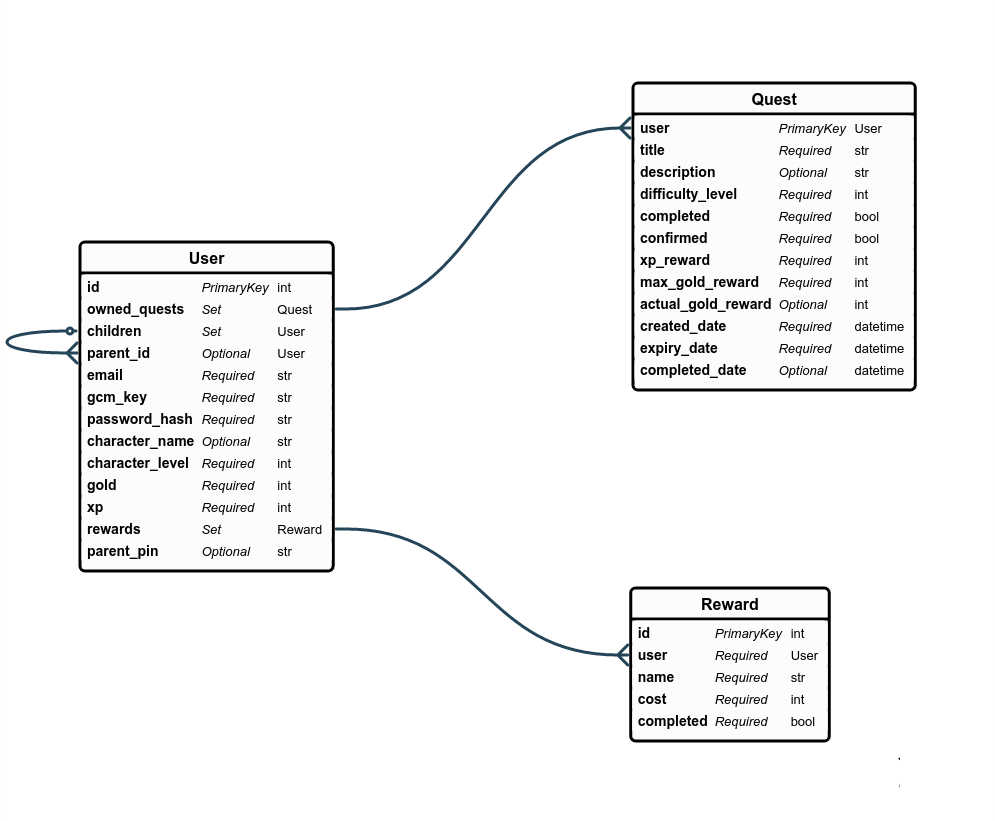
\includegraphics[width=0.75\textwidth]{images/entityRelationshipDiagram.png}
	\caption{Entity-Relationship Diagram}
	\label{fig:ERD}
\end{figure}

I have chosen to create the application in the Android SDK largely due to my previous experience with Java and Android. 
Furthermore, I believe Android is more applicable to the target audience of the app, as Android owns 82.8\% of the smartphone market share as of 2015.
%http://www.idc.com/prodserv/smartphone-os-market-share.jsp
I believe that parents are also more likely to buy their children Android phones than other brands due to the lower price point, making them more appealing when considering the likelihood of them being lost or broken by a child.

For the data analytics, I have opted to use web services written in Flask microframework for python, hosted on a server running Ubuntu Server 14.04. 
I have chosen python due to it's strong backing and community support in data analytics, and is one of the main languages of choice for scientists and statisticians.
The flask framework was chosen specifically as it is very simple to write and host RESTful APIs over the web.

To safely store and version control the code, I used a GitHub private repository to host my code in cloud storage and allow for me to better manage changes to the code-base. 

\section{Aesthetic Design}

\subsection{Wireframes}

\subsection{Android Developer Guidelines}

\section{Usability}

\section{Use Cases}	

\section{Development Style}


%!TEX root = ../main.tex

% 1000-2000 Words

\chapter{Implementation}

\section{Application}
\subsubection{Android}
Android has been chosen for this application due to the large success and market hold of the operating system.

Primarily I will be targeting to support Android versions down to API level 16 (Jelly Bean 4.1).
This decision has been made as figure \ref{fig:AndroidVersions} shows that by supporting this far back, my application will be compatible with over 95\% of current phones. 
Older versions than this will not be targeted, as development and testing time is limited and many features will have to be limited due to lacking functionality within these older versions.

\subsubsection{Material Design}
In order to keep up with a modern and usable design for KidQuest, I have chosen to adhere to the most current standards set by Google for material design.

\subsubsection{Google Cloud Messaging}
The app will be responsible for relaying information between the parent and child clients in a reliable and timely manner.


\subsection{Facebook SDK}
In order to achieve better functionality in the social media features within the app, I will need to gather access to certain information about the user with their strict and explicit permission. 
Tying in the Facebook SDK into the app is the easiest way to gather this information in a secure manner that does not supercede the users wishes.
For example, using the Facebook SDK, I can prompt the user to allow the app permission to gather the users friends list, detect which of them also have used the app and have connected it to facebook and connect the two users as friends within my app.
%TODO: Reword this shit
This technology has strict ethical concerns however, as gathering this information on children has a potential risk for privacy and security concerns, therefore

\subsection{SQLite}

\subsubsection{Object-Relational Mapper}
I chose to use a pre-built Object Relational Mapping library to interface with the database, rather than crafting particular queries on an ad hoc basis.
This was primarily for more ease-of-use purposes than any performance reasons. 
I considered a variety of options for which library to use, initially deciding upon SugarORM due to its very quick learning curve and low use of boilerplate syntax. 

However, ultimately I decided to go with GreenDAO due to more community support - based on GreenDAO having four times the number of community questions on Stack Overflow - and better documentation.
GreenDAO allowed for me generate my MySQL tables, the Java objects and data access object (DAO) patterns by writing out the names of the tables, their properties and their relationships. 

\section{Server}
\subsection{Flask}
For the server-side implementation, I will need tools that allow me to easily create a Web-Service API and provide controlled access to these over the web.
For this task, I have chosen to use Flask as it is well established within the Python community and is incredibly low-effort to set up. 
Flask is suitable for both quick prototyping of web-services and reliable deployment/hosting of functionality over the internet.
By setting up 

\subsubsection{REST vs. SOAP}

\subsubsection{JSON vs. XML}
In order to communicate to the servers web services, I will need to decide upon a message format. 
REST is capable of using both XML and JSON to communicate over the web, 



As the project began it was clear that my initial database/class diagrams were drawn with incorrect assumptions about the project. 
Previously, I have mostly worked on systems that handle many users logging into a web application and designed databases as such. 
However, I did not account for the fact that with an android application, the database only needs to handle one user, which allowed me to use a simpler - less relationship heavy - database design.

\section{Server Rewrite}
When it came to be time to implement the parent app, it was realized that the initial designs for the server were not suitable for KidQuest.
I had initially tried to implement all workflows into the app and store the quests on the client end. 
The plan was then to send the quests to the parent phone using Google Cloud Messaging (GCM) and have them send back which quests were completed.
However, GCM was not suitable for moving the quests reliably and I found that it was too likely that information would be lost or become out of sync between parent and child devices.

Therefore, I decided to push most of the data and functionality to the server-side and have the app interact with the server to perform actions.
I still chose to use GCM for communicating from the server to a client in order to push notifications when tasks are confirmed or completed.

Making the move to server-side implementation did have two main consequences. 
Firstly, users would now require an internet connection to use the app so that it is able to communicate with the server.
This may cause an issue for users who have limited data plans on their phone contracts, however, as the app only communicates using JSON web service requests, data usage is kept to a minimum as requests are only a few kilobytes at a time.
Also, these users will often be conscious about their data usages anyway and will use android settings to restrict data, or only use the app on WiFi. 
Secondly, I would need to have increased security requirements surrounding the data, making sure that it is sufficiently encrypted during transfer to the server, and that the data stored on the server itself is protected as well.
All users were now required to create an account with the server in order to use the app, as the server needed to store the data on it's end rather than on the users' phone.

However, making the move to server-side functionality offers many benefits also.
By implementing everything server-side, the app has become significantly more portable. 
As all functionality rests in the server, any alternative apps - such as iOS or a web app - would be trivial to create as they only have to tie into the existing API, and the only code that would need to be created for these apps would be code to simply send and receive web service requests to the API.
Furthermore, it would also create the ability for the app to easily work between users using different versions. 
i.e. An parent using iOS would be able to monitor a child using an Android phone.

To handle logins securely, I implemented a token-based authentication system within the server. 
Upon their first request, the user submits their username and password within a HTTP POST request to the endpoint `api/token'.
The server then sends back an encrypted token that is derived out of various attributes of their account, which the user client stores.
The app will then authenticate itself with the server for every future request using this token.
This offers the main benefit that the app only has to store the token and not the username and password, which would leave it vulnerable to other (malicious) apps accessing it.
The app will also not have to send their username and password with each request that it makes to the API, minimizing the risk of the password within the request being intercepted in transport.
The password is only stored within the server, which has securely encrypted it with a salted hash.


Separating child and parent users was a mistake.

Interestingly, \cite{4597151} also states that testing a program tells us `little about its quality', arguing that the quality of a test case far outweighs sheer quantiy of tests.

\section{Test-Driven Development}
In the creation of a REST API, it is much easier to develop a test plan due to the clearly laid out workflow of the user. From the server's point of view, there are only a handful of requests that a user can make, and only a handful of tests for those requests. Before writing each endpoint of the server, I 

\section{Functional Testing}

\section{Unit Testing}

\section{Usability Testing}

\section{Beta Testing}

%!TEX root = ../main.tex
\chapter{Conclusion}

Lorem ipsum dolor sit amet, consectetur adipisicing elit, sed do eiusmod tempor incididunt ut labore et dolore magna aliqua. 
Ut enim ad minim veniam, quis nostrud exercitation ullamco laboris nisi ut aliquip ex ea commodo consequat. 
Duis aute irure dolor in reprehenderit in voluptate velit esse cillum dolore eu fugiat nulla pariatur. 
Excepteur sint occaecat cupidatat non proident, sunt in culpa qui officia deserunt mollit anim id est laborum.


%\nocite{*} %Take this out if you don't want it to show all the references and only the ones you've referenced 
\bibliography{references}

\begin{appendices}
\end{appendices}


\end{document}